\section{\color[rgb]{0.2,0.4,0.6} {第一章 Latex的插图与项目符号}}
\subsection{行间距}
\begin{spacing}{2.0} %行间距变为double-space
\paragraph{ \ \ } 在这章介绍如何创建 Qt 的对话框。对话框是程序和用户交互的桥梁,提供了程序和用户之间对话的一种方式。
很多程序都是由一个主窗口,在这个主窗口中包含一个菜单条,多个工具条,和足够多
的对话框。也有些程序本身就是一个对话框,直接相应用户的输入请求。
\par 本章中我们首先会用代码的方式创建我们的第一个对话框,然后用 Qt Designer 工具
创建对话框。Qt Designer 是一个可视化的工具,用它可以更快的创建,修改对话框。
\end{spacing}
\subsection{插图}

	
\begin{figure}[!htb] %图片默认会出现在一页的最顶部,通过参数进行更改,h代表here,放不下就放到top,再放不下就放到bottom
\begin{minipage}[t]{0.48\linewidth} %b表示标题底端对齐,t表示按标题顶端对齐,c表示中间对齐
	\centering %后面的内容全部居中
	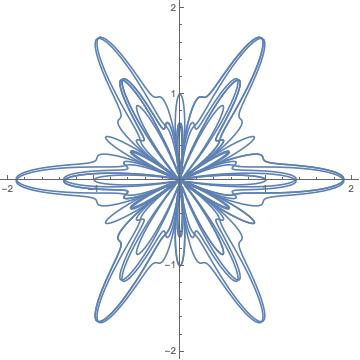
\includegraphics[scale=0.48]{six.jpg} %插入图片并设置缩放,可使用scale=0.x,或者width=0.x乘\textwidth(文字宽度)
	\caption{六角星图}
\end{minipage}
\hfill
\begin{minipage}[t]{0.48\linewidth}
	\centering %后面的内容全部居中
	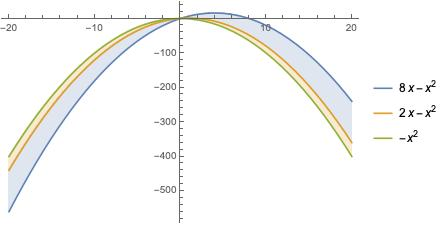
\includegraphics[scale=0.48]{ploy.jpg} %插入图片并设置缩放,可使用scale=0.x,或者width=0.x乘\textwidth(文字宽度)
	\caption{三条线的图}	
\end{minipage}
	
\end{figure}


\subsection{项目符号}
\begin{itemize} %项目符号
	\item yes
\end{itemize}

\begin{enumerate}%项目符号
	\item[一.] A
\end{enumerate}

\subsection{表格}
\begin{table}[!htb] %表格
\centering
	\begin{tabular}{|c|l|r|}
		\hline
		paper & pencil & ruler \\
		\hline
		10\$ & 20\$ & 30\$ \\
		\hline
	\end{tabular}
	\caption{购物表}
\end{table}


\vskip 3 cm %跳过x cm的间距。

\newpage
